\section{Résolution d'un problème (4 points)}

Par mégarde, on a remplacé un fusible de 5 $A$ par un fusible de 10 $A$ dans le tableau électrique de la voiture. Qu'a-t-il pu arriver à la voiture Tesla pour qu'elle prenne feu ?


	\begin{doc}[h!]
		\caption{Voiture électrique Tesla S\textregistered}
		
		\begin{center}
			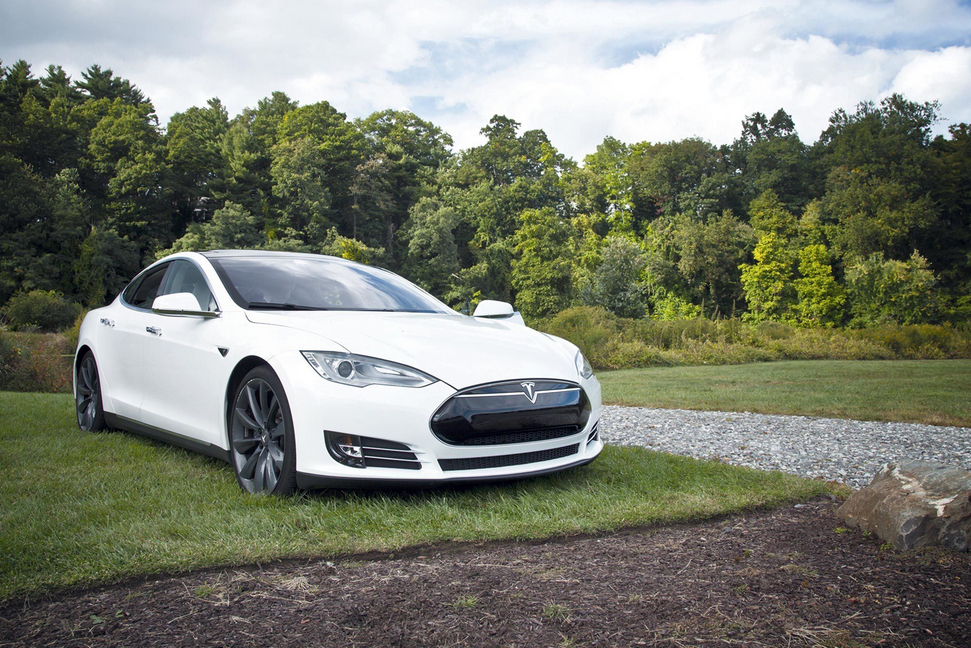
\includegraphics[scale=0.35]{img/tesla}
		\end{center}
	\end{doc}
	
	\begin{doc}[h!]
		\caption{D'après l'Est Républicain, 17 aout 2016 }
		
		<< Une voiture du fabricant américain de véhicules électriques Tesla Motors (modèle S90 D) a pris feu spontanément ce lundi à Bayonne à l'occasion de journées promotionnelles.>>
	\end{doc}




\begin{doc}[h!]
	\caption{Schéma de différents fusibles à lames}
	
	\begin{center}
		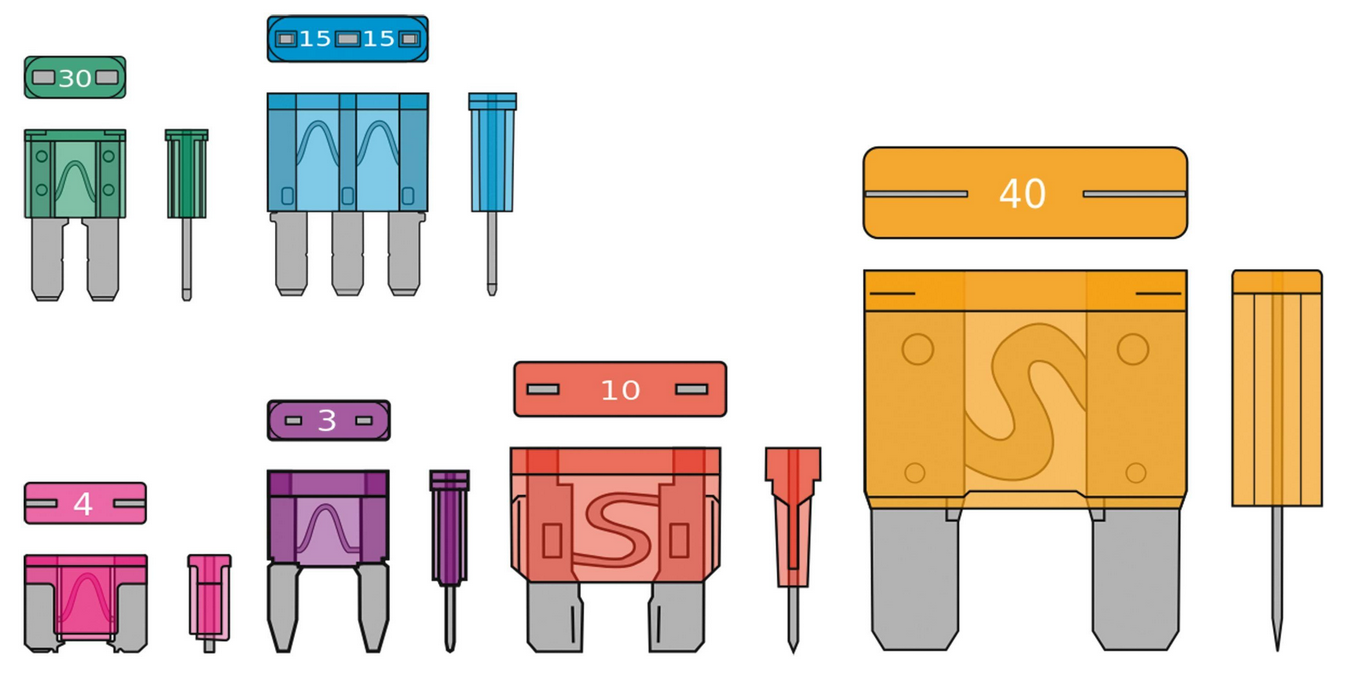
\includegraphics[scale=0.35]{img/fusibles}
	\end{center}
	
	Pour protéger les circuits électriques des véhicules, on utilise des fusibles. Ceux-cis fondent en cas d'intensité trop forte : le circuit est alors ouvert.
\end{doc}